%%%%%%%%%%%%%%%%%%%%%%%%%%%%%%%%%%%%%%%%%%%%%%%%%%%%%%%%%%%%%%%%%%%%%%%%%%%
%%%             DESCRICOES TEORICAS E FERRAMENTAS BASICAS               %%%
%%%%%%%%%%%%%%%%%%%%%%%%%%%%%%%%%%%%%%%%%%%%%%%%%%%%%%%%%%%%%%%%%%%%%%%%%%%

\setlength{\parskip}{0.3cm}

\chapter{Fundamentação Teórica}~\label{ch:fundamentacao}
% FAZER
% Analisar e reescrever introdução da fundamentação teórica
A análise de genes virais baseada em codons é um campo interdisciplinar que exige uma sólida compreensão de diversos conceitos e técnicas. Neste capítulo, exploraremos a fundamentação teórica necessária para a compreensão completa do projeto. Começaremos por abordar os princípios fundamentais da genética viral, discutindo o que é um genoma viral e o papel dos genes em vírus. Em seguida, examinaremos detalhadamente o código de codificação genética fornecida pela \gls{iupac}, que é essencial para traduzir sequências de nucleotídeos em sequências de aminoácidos.

% FAZER
% Reescrever essa parte, tirando o DSR que está no outro capítulo
Este capítulo também destacará a importância da filogenética na classificação de genes virais e como as árvores filogenéticas são construídas com base em informações genéticas. Além disso, discutiremos a metodologia de Design Science Research (DSR), que serve como um guia metodológico para o desenvolvimento da nossa ferramenta.

Para entender completamente os métodos e resultados apresentados nos capítulos subsequentes, é crucial absorver os conceitos apresentados aqui. O conhecimento teórico sólido proporcionará a base necessária para a análise crítica do desenvolvimento da nossa ferramenta de análise de genes virais baseada em codons.

Vamos começar esta jornada pela fundamentação teórica que sustenta o projeto, garantindo uma compreensão sólida e fundamentada de cada passo subsequente.

\section{Biologia Molecular}
A Biologia Molecular é um ramo da biologia que lida e investigas os processos e mecanismos moleculares relacionados à estrutura, função e interações das biomoléculas presentes nos organismos vivos~\cite{alberts_biologia_2017}. Consiste principalmente em estudar as interações entre os vários sistemas da célula, partindo da relação entre o \gls{dna}, \gls{rna} e a síntese de proteínas, e o modo como essas interações são reguladas.

É fundamental entender a estrutura do \gls{dna} apresentada na Figura~\ref{fig:estruturaDNA}. Está é uma molécula em forma de dupla hélice que carrega a informação genética em organismos vivos. Ela é composta por duas cadeias polinucleotídicas complementares enroladas em torno de um eixo central. Cada cadeia é composta por uma sequência de nucleotídeos, que consistem em uma pentose (a desoxirribose), um grupo fosfato e uma base nitrogenada que pode ser \gls{adenina}, \gls{timina}, \gls{citosina} ou \gls{guanina}. A maior parte dos organismos carrega suas informações genéticas no \gls{dna}, mas alguns vírus carregam essa informação no \gls{rna}, que possui as mesma bases do \gls{dna} só substituindo a \gls{timina} pela \gls{uracila}~\cite{genetica_peter_2017}.

\begin{figure}[htb]
  \centering
  \caption{Estrutura do DNA.}
  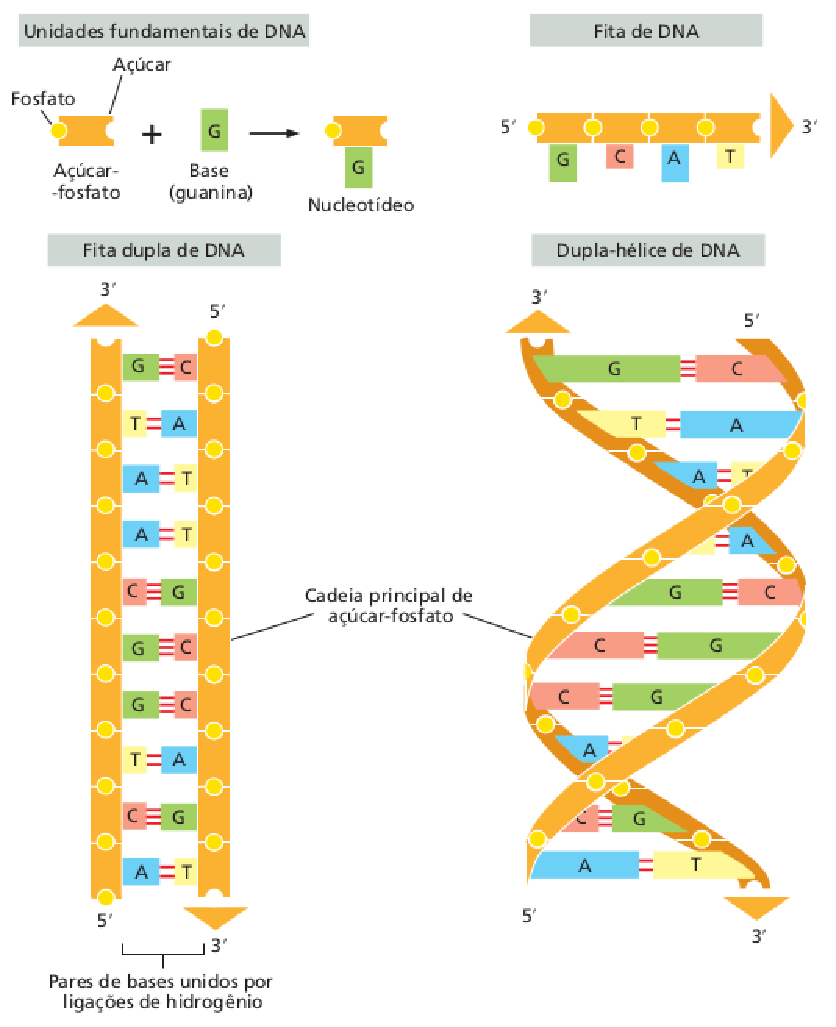
\includegraphics[scale=0.6]{figuras/estruturaDNA_02.pdf}
  \fonte{Retirada de \textit{\citeauthor{alberts_biologia_2017}}}~\label{fig:estruturaDNA}
\end{figure}

Além das bases nitrogenadas principais já apresentadas (\gls{adenina}, \gls{timina}, \gls{citosina} e \gls{guanina}), a \gls{iupac} que é uma organização não governamental internacional dedicada ao avanço da química, desenvolveu também outras codificações, conhecida como \textit{IUPAC Nucleotide Code}, para representar de maneira padronizada as bases nitrogenadas encontradas nas moléculas de ácido nucleico. Também são apresentadas outras letras que representam pares de bases ou misturas específicas, a letra ``N'' que é usada para representar uma base desconhecida ou não especificada e os símbolos de ``.'' ou ``-'', conhecidos como ``GAP'', ou seja, representa onde há uma base identificável ou onde a informação é faltante. As mesmas são apresentadas na tabela~\ref{tab:iupacNucleotideCode} a seguir.

\begin{table}[htb]
  \caption{\textit{IUPAC Nucleotide Code}.}
  \begin{center}
    \begin{tabular}{c|c}
      \hline
      Base             & IUPAC Nucleotide Code    \\
      \hline
      Adenina          & A                        \\
      Citosina         & C                        \\
      Guanina          & G                        \\
      Timina           & T                        \\
      Uracila          & U                        \\
      A ou G           & R                        \\
      C ou T           & Y                        \\
      A ou C           & M                        \\
      G ou T           & K                        \\
      G ou C           & S                        \\
      A ou T ou G      & W                        \\
      C ou G ou T      & B                        \\
      A ou C ou T      & D                        \\
      A ou G ou T      & H                        \\
      C ou G ou A      & V                        \\
      A ou C ou G ou T & N                        \\
      GAP              & \textbf{.} ou \textbf{-} \\
      \hline
    \end{tabular}
  \end{center}
  \fonte{Criada pelo autor.}\label{tab:iupacNucleotideCode}
\end{table}

% FAZER
% Corrigir/Complementar a definição de genoma e gene
% Comparar o genoma humano com o genoma viral em relação a quantidade de pares de bases
% https://www.genome.gov/genetics-glossary/Genome REF para imagens
O conjunto completo de material genético contido em um organismo, seja ele um vírus, uma bactéria, uma planta ou um animal é conhecido como genoma. Ele abrange todas as informações genéticas necessárias para o desenvolvimento, funcionamento e reprodução do organismo. O genoma é composto por sequências de \gls{dna} que carregam as instruções para a síntese de proteínas e regulam várias funções celulares~\cite{alberts_biologia_2017,genetics_benjamin_2016}. A análise do genoma desempenha um papel fundamental na genética, na biologia molecular e na compreensão da hereditariedade e da evolução.~\cite{alberts_biologia_2017}

As informações contidas no \gls{dna} são copiadas em uma molécula de \gls{rna}, esse processo é conhecido como transcrição. A transcrição ocorre no núcleo das células e envolve a separação das duas fitas do \gls{dna} e o pareamento de nucleotídeos complementares para sintetizar uma molécula de \gls{mrna}. O \gls{mrna} é uma cópia do DNA que carrega a sequência de bases nitrogenadas correspondente a um gene específico.
Após isso, ocorre o processo de tradução onde a sequência de bases nitrogenadas do \gls{mrna} é utilizada para sintetizar proteínas. A tradução ocorre nos ribossomos, presentes no citoplasma celular. Durante a tradução, o \gls{mrna} é lido em grupos de três bases, chamados de códons. Os códons são sequências de três nucleotídeos consecutivos no RNA que correspondem a um aminoácido específico. Existem 64 códons possíveis, correspondentes a 20 aminoácidos diferentes como apresentado na Figura~\ref{fig:tabelaCodons}, além de sinais de início e parada da tradução. A tradução é o processo pelo qual a sequência de códons no RNA é utilizada para sintetizar proteínas. Durante a tradução, os códons são reconhecidos por moléculas de RNA transportador (tRNA) que trazem os aminoácidos correspondentes.
\begin{figure}[htb]
  \centering
  \caption{Tabela de Códons.}
  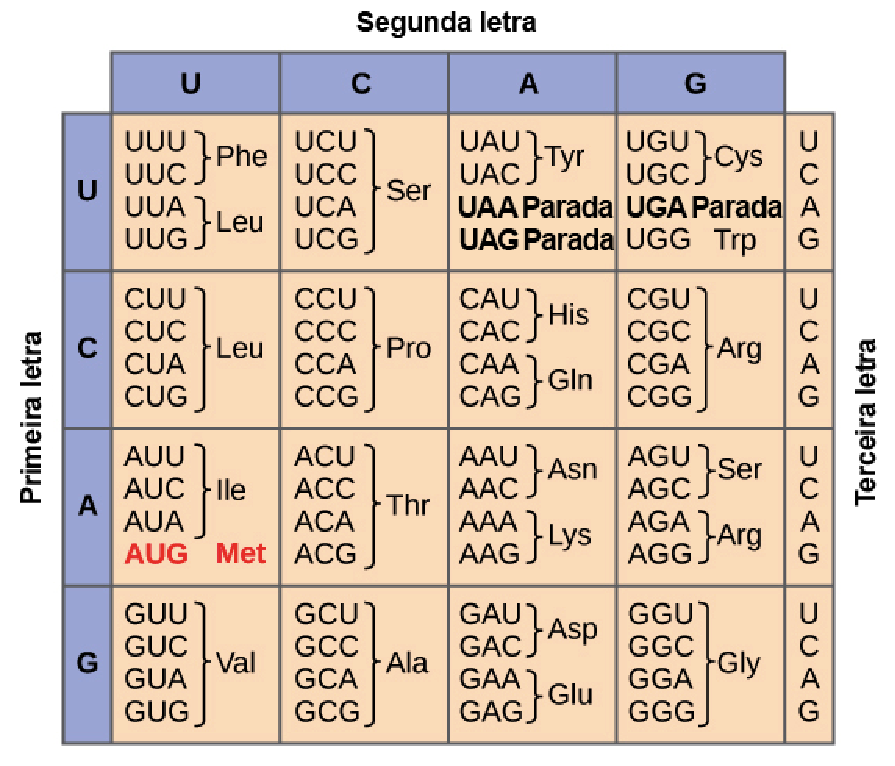
\includegraphics[scale=0.6]{figuras/tabelaCodons.pdf}
  \fonte{Adaptada de \citeauthor{openstax-genetic-code}}~\label{fig:tabelaCodons}
\end{figure}

A relação entre os códons, o DNA e o RNA é crucial para a síntese de proteínas e a expressão genética. O sequenciamento do DNA e a identificação dos códons correspondentes permitem a inferência das sequências de aminoácidos nas proteínas codificadas por um determinado gene.
Cada códon especifica um aminoácido distinto. Os aminoácidos são transportados para o ribossomo por moléculas de \gls{trna}, que possuem um anticódon complementar ao códon do \gls{mrna}. À medida que o ribossomo percorre o \gls{mrna}, os aminoácidos são ligados em uma sequência específica, formando uma cadeia polipeptídica que será dobrada e modificada para se tornar uma proteína funcional~\cite{alberts_biologia_2017}.

% FAZER
% Sequenciamento genético (Como são obtidas as sequências) De forma bem sucinta
Para determinar a ordem exata dos nucleotídeos em uma molécula de \gls{dna} ou \gls{rna} é realizada uma técnica conhecida como sequenciamento genético. Existem várias técnicas de sequenciamento, cada uma com suas vantagens e desvantagens, sendo as mais notáveis o sequenciamento de Sanger, o \gls{ngs} e o sequenciamento de terceira geração.~\cite{nanopore_sequence_jain_2016,dna_sequence_sanger_1977,next_generation_sequence_goodwin_2016}

\section{Vírus}

Os vírus são agentes infecciosos que possuem uma estrutura viral que varia entre os seus diferentes tipos, mas que de modo geral é composta por uma cápsula proteica chamada capsídeo, que envolve o material genético viral, que pode ser \gls{dna} ou \gls{rna}. O capsídeo pode apresentar diferentes formas, como hélices, icosaedros ou formas complexas. Além do capsídeo, alguns vírus possuem uma camada lipídica chamada envelope viral, que é derivada da membrana da célula hospedeira e contém glicoproteínas virais que são importantes para a entrada do vírus nas células hospedeiras~\cite{david_virology_2022}.
O ciclo e vida viral é conjunto de etapas que um vírus passa para se reproduzir e infectar novas células. Esse ciclo pode variar entre diferentes tipos de vírus, mas geralmente envolve as seguintes etapas~\cite{alberts_molecular_2002}:

\begin{enumerate}
  \item \textbf{Adsorção:} o vírus se liga especificamente a receptores na superfície da célula hospedeira.
  \item \textbf{Penetração:} o vírus é internalizado na célula hospedeira, liberando seu material genético.
  \item \textbf{Replicação e síntese de proteínas virais:} o material genético viral é transportado para os ribossomos da célula hospedeira, replicado e transcritas em moléculas de \gls{mrna}, que são utilizadas para a síntese de proteínas virais.
  \item \textbf{Montagem:} as proteínas virais se unem para formar novas partículas virais.
  \item \textbf{Liberação:} as novas partículas virais são liberadas da célula hospedeira, para a montagem de novos vírus e para a modificação do ambiente celular para garantir a sua replicação.
        % \item \textbf{Liberação:} as novas partículas virais são liberadas da célula hospedeira, podendo ocorrer por lise celular ou por brotamento
\end{enumerate}

\subsection{SARS-CoV-2}

O SARS-CoV-2 é um vírus da família Coronaviridae, que causa a doença chamada \gls{covid19}. Ele foi identificado pela primeira vez em dezembro de 2019 na cidade de Wuhan, na província de Hubei, na China, e desde então se espalhou para todo o mundo, resultando em uma pandemia global~\cite{zhu_novel_2020,wu_coronavirus_2020}.

O SARS-CoV-2 possui uma estrutura viral apresentada na Figura~\ref{fig:estruturaCoronavirus}, característica dos coronavírus. Ele é composto por uma partícula viral esférica, com um envelope lipídico que envolve seu material genético. A estrutura do vírus inclui proteínas de espículas na sua superfície, conhecidas como proteína spike (S). Além disso, o SARS-CoV-2 possui proteínas de membrana (M), envelope (E) e nucleocapsídeo (N), que desempenham papéis importantes na estrutura e na replicação viral.

\begin{figure}[htb]
  \centering
  \caption{Estrutura do coronavírus.}
  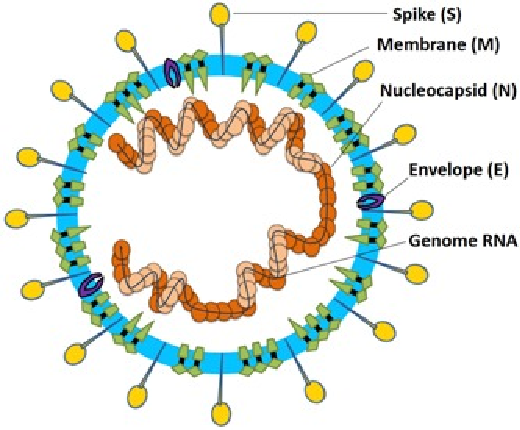
\includegraphics[scale=0.8]{figuras/estruturaSarsCov2.pdf}
  \fonte{Retirada de \textit{\citeauthor{li_coronavirus_2020}}}~\label{fig:estruturaCoronavirus}
\end{figure}

% SPIKE
A proteína Spike (S) do vírus SARS-CoV-2 é uma das principais proteínas de superfície do vírus e desempenha um papel crucial na infecção das células hospedeiras. Ela é uma glicoproteína que forma estruturas semelhantes a espículas na superfície do vírus, dando-lhe uma aparência coroada. A proteína Spike é o alvo principal das respostas imunes do hospedeiro e é fundamental para a ligação do vírus às células humanas e sua subsequente entrada.

A proteína Spike é composta por três domínios principais: o domínio de ligação ao receptor (RBD -~Receptor-Binding Domain), o domínio de fusão (FD -~Fusion Domain) e o domínio N-terminal (NTD -~N-Terminal Domain). O RBD é particularmente importante, pois é responsável pela interação com o receptor da enzima conversora de angiotensina 2 (ACE2) nas células hospedeiras humanas. Essa interação é crucial para a entrada do vírus nas células.
% Apresentar imagem específica da SPIKE

A estrutura da proteína Spike é altamente dinâmica e pode mudar de conformação para facilitar a fusão da membrana viral com a membrana da célula hospedeira, permitindo assim a entrada do vírus. Essa capacidade de mudança conformacional torna a proteína Spike um alvo promissor para o desenvolvimento de vacinas e terapias antivirais.

Estudos detalhados da proteína Spike são essenciais para compreender a patogenicidade do vírus SARS-CoV-2 e para o desenvolvimento de estratégias terapêuticas eficazes. Além disso, mutações na proteína Spike têm sido identificadas como uma das principais causas de variantes do vírus, o que destaca ainda mais a importância de sua investigação contínua.
% SPIKE

\subsubsection{Nomenclaturas de Linhagens do SARS-CoV-2}
A nomenclatura das linhagens do \gls{sarscov2} é uma parte crucial na classificação e rastreamento das diferentes variantes do vírus. Duas das principais nomenclaturas usadas para descrever essas linhagens são a nomenclatura \gls{pango} e a nomenclatura da \gls{who}. Essas nomenclaturas são usadas para descrever as diferentes variantes do vírus com base em suas características genéticas e filogenéticas.

A nomenclatura \gls{pango} é uma abordagem baseada na filogenia para nomear e rastrear as linhagens do \gls{sarscov2}. Ela atribui um nome único a cada linhagem com base em sua posição na árvore filogenética do vírus. Isso permite uma identificação clara das diferentes linhagens e ajuda na compreensão de como o vírus está evoluindo ao longo do tempo.~\cite{pango_rambaut_2020}

Já a \gls{who} também desenvolveu sua própria nomenclatura para classificar as variantes do \gls{sarscov2}. Essa nomenclatura envolve a utilização de letras gregas em ordem alfabética (Alpha, Beta, Gamma, Delta, etc.) e foi aplicada para evitar a estigmatização de locais geográficos ou populações.~\cite{who_variants} Além disso, a \gls{who} também dividiu as variantes em 3 (três) grupos distintos: \gls{vum}, \gls{voi} e \gls{voc}.

A \gls{vum} é um termo usado para sinalizar às autoridades de saúde pública que uma variante do SARS-CoV-2 pode exigir atenção e monitoramento priorizados. O principal objetivo desta categoria é investigar se esta variante (e outras intimamente relacionadas com ela) pode representar uma ameaça adicional à saúde pública global em comparação com outras variantes em circulação.
Já a \gls{voi}, é um termo usado para descrever uma variante do SARS-CoV-2 com alterações que afetam o comportamento do vírus ou seu impacto potencial na saúde humana. Isto pode incluir, por exemplo, a sua capacidade de propagação, a sua capacidade de causar doenças graves ou a facilidade com que pode ser detectada ou tratada. Um VOI também pode ser identificado porque tem uma maior capacidade de propagação quando comparado com outras variantes em circulação, sugerindo um potencial risco emergente para a saúde pública global. Por fim, a \gls{voc} é um termo que descreve uma variante do SARS-CoV-2 que atende à definição de \gls{voi}, mas também atende a pelo menos um dos seguintes critérios quando comparado com outras variantes\cite{who_variants}:
\begin{itemize}
  \item pode causar uma mudança prejudicial na gravidade da doença.
  \item   pode ter um impacto substancial na capacidade dos sistemas de saúde de prestar cuidados a pacientes com COVID-19 ou outras doenças e, portanto, exigir grandes intervenções de saúde pública.
  \item há uma diminuição significativa na eficácia das vacinas disponíveis na proteção contra doenças graves.
\end{itemize}

A tabela~\ref{tab:nomenclaturaPangoWho} apresentada a seguir, contem as \gls{voc} \textit{Alpha, Beta, Gamma, Delta e Omicron}\footnote{Essa variante possui sublinhagens }, com as suas respectivas nomenclaturas \gls{pango} e \gls{who}

\begin{table}[htb]
  \caption{Variantes VOC e suas Nomenclaturas \textit{PANGO e WHO}.}
  \begin{center}
    \begin{tabular}{c|c}
      \hline
      Nomenclatura WHO & Nomenclatura PANGO \\
      \hline
      Alpha            & B.1.1.7            \\
      Omicron          & B.1.1.529          \\
      Beta             & B.1.351            \\
      Delta            & B.1.617.2          \\
      Gamma            & P.1                \\
      \hline
    \end{tabular}
  \end{center}
  \fonte{Criada pelo autor.}\label{tab:nomenclaturaPangoWho}
\end{table}

\section{Bioinformática}
% Alinhamento de Sequências, Análise de Genomas Virais, Análise de Genomas Virais, Análise de Expressão Gênica, Ferramentas de Bioinformática (Algoritmos de Alinhamento e Algoritmos de reconstrução de árvores)
A bioinformática é um campo interdisciplinar que aplica técnicas de ciência da computação e estatística para entender e interpretar dados biológicos. Essa área surgiu com o advento das tecnologias de sequenciamento de DNA e tem se expandido para abranger diversos aspectos da biologia molecular e genômica. Vamos explorar os principais domínios da bioinformática:

% FAZER Verificar se está correto ou não e adicionar as referências
Alinhamento de Sequências:
O alinhamento de sequências é uma tarefa central na bioinformática, permitindo comparar e identificar similaridades entre sequências biológicas. Algoritmos como Needleman-Wunsch e Smith-Waterman são usados para alinhamentos globais e locais, respectivamente. Ferramentas populares incluem o BLAST (Basic Local Alignment Search Tool) e o ClustalW.

Análise de Genomas:
A análise de genomas visa entender a organização, função e evolução dos genes em um organismo. Ferramentas como Artemis e o Ensembl Genome Browser facilitam a navegação e interpretação de genomas completos.

Análise de Expressão Gênica:
Métodos como RNA-Seq e microarrays são usados para medir a expressão de genes em diferentes condições. Softwares como DESeq2 e edgeR realizam análise diferencial de expressão, identificando genes com níveis significativamente diferentes de expressão.

Filogenética:
A filogenética estuda as relações evolutivas entre organismos. Métodos como Máxima Verossimilhança (RAxML), Métodos Bayesianos (MrBayes) e Métodos de Distância (Neighbor-Joining) são utilizados para reconstruir árvores filogenéticas.

Estrutura de Proteínas:
Ferramentas como o Phyre2 e o SWISS-MODEL permitem a modelagem e predição da estrutura tridimensional de proteínas, proporcionando insights sobre sua função.

Metagenômica:
A metagenômica analisa comunidades microbianas em amostras ambientais. Ferramentas como QIIME e MEGAN auxiliam na análise de dados de sequenciamento de amplicons e metagenomas.
\section{Filogenia}
% FAZER
% Escrever sobre Modelos Evolutivos
% GTR Generalized time Reversible

A filogenia é uma disciplina da biologia que estuda as relações evolutivas entre organismos, buscando reconstruir a história evolutiva e a ancestralidade comum. A filogenética molecular é uma abordagem utilizada para inferir a filogenia com base em informações moleculares, como sequências de \gls{dna}, \gls{rna} e proteínas\cite{felsenstein_inferring_2004}.

A construção de árvores filogenéticas é um aspecto fundamental da filogenética molecular. Existem vários métodos utilizados para construir árvores filogenéticas, que podem ser classificados em dois grupos principais: métodos baseados em distância e métodos baseados em caracteres.
Os métodos baseados em distância medem a similaridade ou a dissimilaridade entre sequências moleculares e constroem árvores filogenéticas com base nessas medidas. Alguns exemplos de métodos baseados em distância incluem o método de Neighbor Joining (NJ) e o método de Mínima Evolução (ME).
Por outro lado, os métodos baseados em caracteres analisam as mudanças nos caracteres moleculares ao longo do tempo para inferir as relações filogenéticas. Exemplos de métodos baseados em caracteres são o método de Máxima Parcimônia (MP) e o método de Inferência Bayesiana\cite{swofford_phylogenetic_1996}.

% Abordagens anteriores em ordem cronológica
Ao longo dos anos, vários métodos utilizados para análise filogenética foram desenvolvidos, logo após, será apresentado alguns dos principais e amplamente utilizados:

\begin{enumerate}
  \item \textbf{Método de reconstrução de árvore filogenética de distância (1957)}: Esse método é baseado na construção de árvores filogenéticas a partir de uma matriz de distâncias que quantifica a diferença evolutiva entre diferentes sequências. A árvore é construída de modo que as sequências mais semelhantes estejam mais próximas umas das outras. Esse método é amplamente utilizado em análises filogenéticas e é uma das técnicas mais antigas~\cite{sokal_statistical_method_1958}.
  \item \textbf{Método de máxima parsimônia (1966)}: A máxima parsimônia busca a árvore filogenética mais simples, ou seja, aquela que requer o menor número de mudanças evolutivas para explicar as sequências observadas. Esse método é baseado no princípio de que a evolução segue o caminho mais econômico, evitando mudanças desnecessárias~\cite{fitch_toward_definition_1971}.
  \item \textbf{Método de máxima verossimilhança (1981)}: O método de máxima verossimilhança estima a árvore filogenética que maximiza a probabilidade de observar as sequências dadas, dadas as hipóteses filogenéticas. Ele é baseado na modelagem estatística da evolução molecular e é amplamente considerado um dos métodos mais precisos para a reconstrução de árvores filogenéticas~\cite{felsenstein_evolutionary_tree_1981}.
  \item \textbf{Método de junção de vizinhos (1987)}: O método Neighbor-Joining é uma técnica de construção de árvore filogenética que se baseia em uma abordagem de aglomeração hierárquica. Ele é amplamente utilizado para criar árvores filogenéticas a partir de matrizes de distância, representando a proximidade evolutiva entre sequências ou espécies. Esse método é especialmente útil para análises de grandes conjuntos de dados e é conhecido por sua eficiência computacional~\cite{saitou_neighbor_1987}. % MÉTODO UTILIZADO NO AGUA!? Junção de Vizinhos / Neighbor-Joining
  \item \textbf{Método de inferência bayesiana (2001)}: A inferência bayesiana combina informações a priori com dados observados para estimar a árvore filogenética mais provável. Ela se baseia no Teorema de Bayes e permite incorporar informações prévias sobre as relações filogenéticas. Esse método é particularmente útil quando se dispõe de conhecimento prévio sobre as relações entre as espécies~\cite{huelsenbeck_bayesian_inference_2001}.
  \item \textbf{Método de coalescência (2004)}: O método de coalescência, também conhecido como filogenia de coalescência, aborda a filogenia a partir do ponto de vista do ancestral comum mais recente. Ele modela a história da população ancestral e como as sequências evoluíram a partir dessa população. Esse método é especialmente útil para analisar sequências de genes individuais~\cite{kingman_coalescent_1982}.
  \item \textbf{Método de redes filogenéticas (2005)}: As redes filogenéticas são uma extensão das árvores filogenéticas que permitem representar relacionamentos mais complexos, como reticulações ou eventos de hibridização. Elas são úteis quando as relações entre as espécies não podem ser adequadamente representadas por uma árvore simples~\cite{huson_phylogenetic_networks_2006}.
  \item \textbf{Método de filogenia de genoma inteiro (2010)}: Esse método se concentra na análise comparativa de genomas completos para inferir relações filogenéticas. Ele utiliza informações genômicas de alta resolução, como sequências de genes e elementos regulatórios, para construir árvores filogenéticas que refletem a evolução das espécies~\cite{eisen_horizontal_gene_transfre_2000}.
\end{enumerate}

\section{Machine Learning}
% Modelo não supervisionado
% Adicionar as referências (Algumas já estão no bibtex)
Machine learning é uma subárea da inteligência artificial que se concentra no desenvolvimento de algoritmos e modelos que permitem a um sistema aprender a partir de dados e realizar tarefas específicas sem ser explicitamente programado~\cite{deeplearning_goodfellow_2016}. Dentro do campo do machine learning, existem duas categorias principais de aprendizado: supervisionado e não supervisionado. Neste contexto, abordaremos a segunda categoria, com ênfase nos modelos não supervisionados.

O aprendizado não supervisionado é uma abordagem de machine learning na qual o algoritmo é treinado em dados não rotulados, ou seja, dados que não têm rótulos ou categorias previamente atribuídos. O objetivo do aprendizado não supervisionado é explorar a estrutura e os padrões subjacentes aos dados sem orientação externa. Isso torna o aprendizado não supervisionado útil para tarefas em que a natureza dos dados é desconhecida, e os padrões emergentes devem ser identificados~\cite{machine_learning_bishop_2006}.

Um dos principais tipos de tarefa no aprendizado não supervisionado é o agrupamento (clustering). Nessa tarefa, o algoritmo identifica grupos ou clusters de dados que compartilham características semelhantes. O objetivo é agrupar dados de acordo com suas propriedades intrínsecas, sem conhecimento prévio das categorias. Algoritmos de clustering, como o K-Means e o Hierarchical Clustering, são amplamente utilizados em campos como biologia, processamento de imagem, análise de dados e muito mais~\cite{machine_learning_bishop_2006}.

O aprendizado não supervisionado é fundamental em diversas aplicações. Na biologia, por exemplo, algoritmos de clustering podem ser usados para identificar grupos de genes que são coexpressos, revelando padrões de regulação genética. Em finanças, a redução de dimensionalidade pode ser aplicada para entender a relação entre diferentes ativos financeiros. Na área de processamento de linguagem natural, o aprendizado não supervisionado é usado para detectar tópicos em grandes volumes de texto~\cite{bioinformatics_david_2004}.


Apesar de sua versatilidade, o aprendizado não supervisionado também apresenta desafios. A interpretação dos resultados pode ser complexa, pois não há rótulos de classe para validar as descobertas. Além disso, a escolha de hiperparâmetros e a avaliação da qualidade do agrupamento ou da redução de dimensionalidade podem ser complicadas.
Em resumo, o aprendizado não supervisionado desempenha um papel fundamental no campo do machine learning, permitindo a extração de informações valiosas de dados não rotulados. Sua capacidade de encontrar estrutura oculta nos dados é crucial em uma variedade de domínios, tornando-o uma ferramenta poderosa na análise e interpretação de informações complexas\cite{learning_kernels_scholkopf_2002}.

\section{Trabalhos Correlatos}

Na busca de trabalhos relacionados, vários métodos foram encontrados, e a seguir são apresentados.

O método de \gls{ml} (ou \textit{Maximum Likelihood}), não é exclusivo da filogenia, mas sim uma abordagem estatística. A sua aplicação em filogenia consiste em avaliar a probabilidade de que o modelo de evolução escolhido gere os dados observados, que são por exemplo, características de um organismo. Essa proposta foi utilizada nos seguintes trabalhos:
\begin{itemize}
  \item \textit{\citeauthor{behl_threat_2022}}
  \item \textit{\citeauthor{fall_genetic_diversity_2021}}
  \item \textit{\citeauthor{shabbir_comprehensive_2020}}
  \item \textit{\citeauthor{hudu_hepatitis_2018}}
  \item \textit{\citeauthor{sallard_tracing_2021}}
  \item \textit{\citeauthor{paez-espino_diversity_evolution_2019}}
  \item \textit{\citeauthor{tang_evolutionary_2021}}
  \item \textit{\citeauthor{cho_analysis_2022}}
\end{itemize}

Já em~\textit{\citeauthoronline{yin_systematic_2019}} e \textit{\citeauthoronline{bedoya-pilozo_molecular_epidemiology_2018}}, foi usada a inferência bayesiana, que é fundamentada no teorema de Bayes, que permite a atualização das probabilidades a priori para probabilidades a posteriori à medida que novas evidências são incorporadas.

Além desses,~\textit{\citeauthor{potdar_phylogenetic_2021}} utilizou a junção de vizinhos (ou \textit{Neighbor-Joining}), que é baseado em uma abordagem heurística que visa construir uma árvore filogenética a partir de uma matriz de distância entre as sequências estudadas. O trabalho de~\citeauthor{lichtblau_alignment-free_2019} expos o Frequency Chaos Game Representation e~\textit{\citeauthor{kim_ngs_2022}} a floresta aleatória. Por fim,~\textit{\citeauthor{dimitrov_updated_2019}} comparou três modelos para reconstrução de árvores filogenéticas: junção de vizinhos; \gls{ml} e inferência bayesiana.